% Created 2019-11-13 Wed 00:45
% Intended LaTeX compiler: pdflatex
\documentclass[presentation]{beamer}
\usepackage[utf8]{inputenc}
\usepackage[T1]{fontenc}
\usepackage{graphicx}
\usepackage{grffile}
\usepackage{longtable}
\usepackage{wrapfig}
\usepackage{rotating}
\usepackage[normalem]{ulem}
\usepackage{amsmath}
\usepackage{textcomp}
\usepackage{amssymb}
\usepackage{capt-of}
\usepackage{hyperref}
\institute{Universidad Nacional Autónoma de México}
\usetheme{metropolis}
\usecolortheme{}
\usefonttheme{}
\useinnertheme{}
\useoutertheme{}
\author{Adrián Antonio Rodríguez Pié}
\date{21 de noviembre de 2019}
\title{Implementación de redes neuronales convolucionales para el meta-análisis de acoplamientos moleculares de complejos proteína-ligando}
\AtBeginSection{\frame{\sectionpage}}
\metroset{block=fill}
\hypersetup{
 pdfauthor={Adrián Antonio Rodríguez Pié},
 pdftitle={Implementación de redes neuronales convolucionales para el meta-análisis de acoplamientos moleculares de complejos proteína-ligando},
 pdfkeywords={},
 pdfsubject={},
 pdfcreator={Emacs 27.0.50 (Org mode 9.1.9)},
 pdflang={English}}
\begin{document}

\maketitle
\begin{frame}{Outline}
\tableofcontents
\end{frame}



\section{Sobre proteínas}
\label{sec:org9c1b525}
\begin{frame}[label={sec:orgd8c98ff}]{Proteínas}
\begin{block}{Orígen}
Originado del griego \emph{proteios} que significa "primario"
o "de primer orden".
\pause
\end{block}
\begin{block}{Definición (según la \alert{RAE})}
Sustancia constitutiva de la materia viva, formada
por una o varias cadenas de aminoácidos.
\end{block}
\end{frame}
\begin{frame}[label={sec:orgdb416c6}]{Ligandos}
\begin{itemize}
\item Un \alert{ligando} es una molécula que se une a otra molécula específica, en algunos casos mandando una señal en el proceso.
\pause
\item Estos ligandos interactuan con moleculas objetivo (usualmente otras proteínas). Son a estas proteínas a las que llamamos \alert{receptores} o \alert{residuos}.
\end{itemize}
\end{frame}
\begin{frame}[label={sec:orgb6d1281}]{Docking}
\begin{block}{Acoplamiento molecular}
Método cuyo objetivo es predecir los estados tanto estructurales,
llamadas \alert{poses}, como energéticos, prediciendo la afinidad del enlace
entre moléculas.
\begin{center}
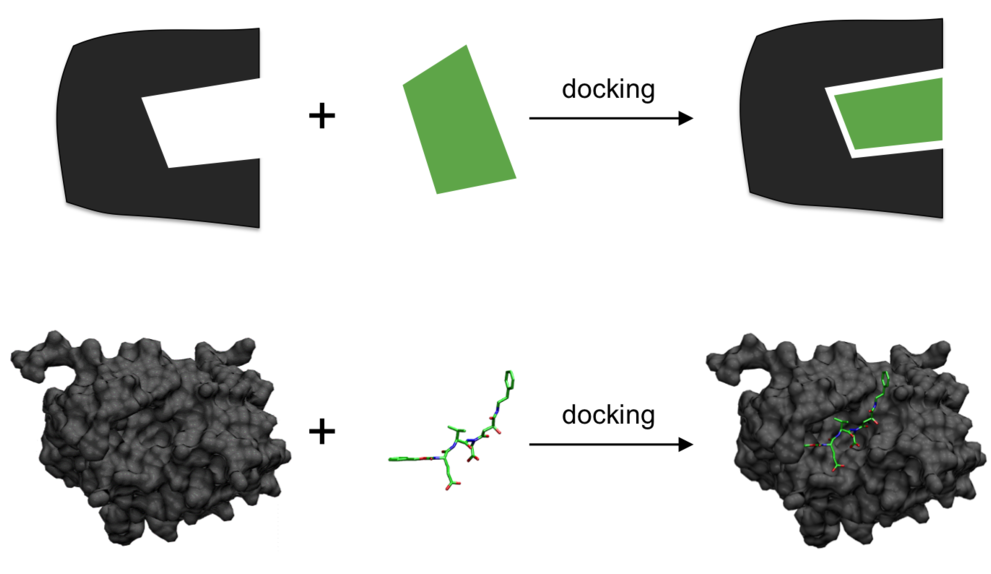
\includegraphics[width=.9\linewidth]{images/docking.png}
\end{center}
\end{block}
\end{frame}
\begin{frame}[label={sec:orgbb53821}]{Pasos del docking}
\begin{center}
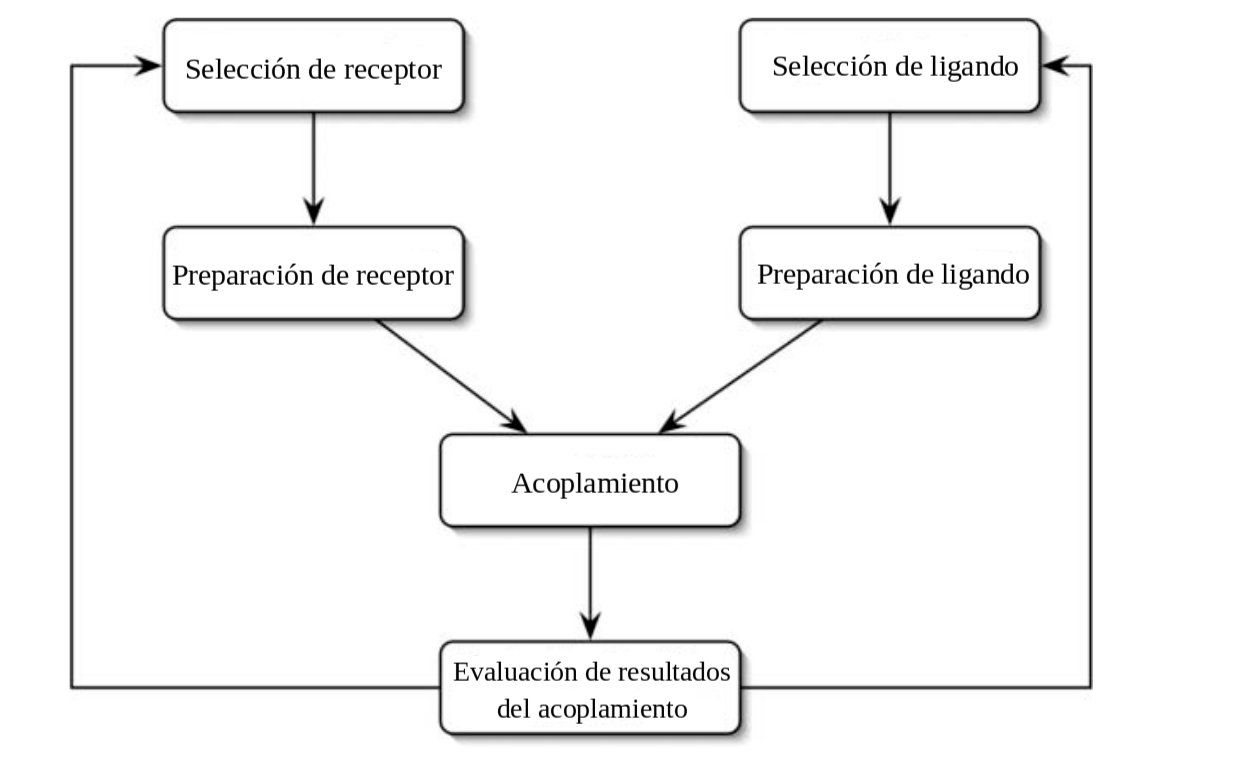
\includegraphics[width=.9\linewidth]{images/docking_steps.png}
\end{center}
\end{frame}
\section{Sobre inteligencia artificial}
\label{sec:org531e1ff}
\begin{frame}[label={sec:orgce5c944}]{La prueba de Turing}
\begin{center}
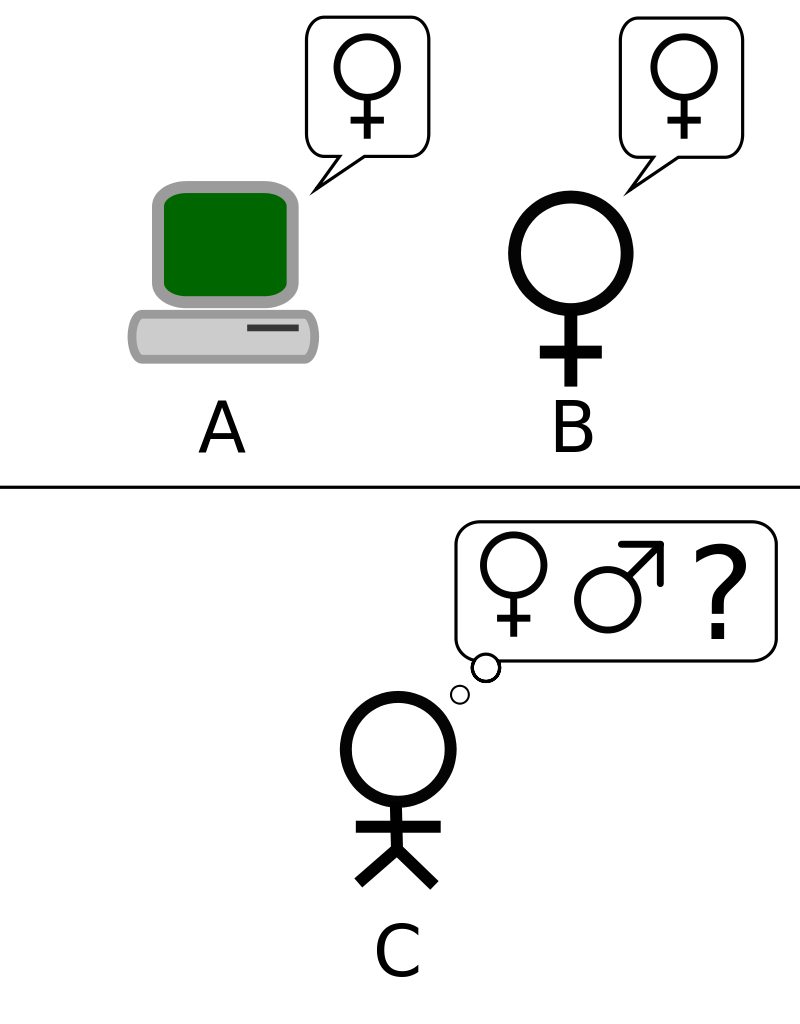
\includegraphics[width=170px]{images/turing-test.png}
\end{center}
\end{frame}
\begin{frame}[label={sec:org6ab5377}]{IA y agentes}
\begin{block}{Inteligencia artrificial}
\alert{\alert{Agentes racionales}} que, mediante \alert{\alert{sensores}}, pueden
percibir su \alert{\alert{entorno}} y actuar sobre él a partir de un
sistema de decisión.
\pause
\end{block}
\begin{block}{Agentes}
Máquina compuesta por un conjunto finito de estados, cuyas
transiciones están dadas por reglas de inferencias.
\end{block}
\end{frame}
\section{Sobre redes y neuronas}
\label{sec:org893ada1}
\begin{frame}[label={sec:org11e3f0a}]{Inspiración en la biología}
\begin{center}
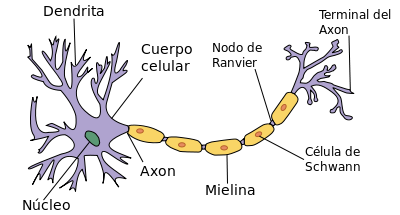
\includegraphics[width=.9\linewidth]{images/neurona.png}
\end{center}
\end{frame}

\begin{frame}[label={sec:orgb2cd66f}]{El perceptrón}
\begin{block}{Definiciónes}
\begin{itemize}
\item \alert{x} \(\in \mathbb{R}^n\) (muestra)
\item \alert{w} \(\in \mathbb{R}^n\) (vector de pesos)
\item \alert{\(\theta\)} \(\in \mathbb{R}^n\) (umbral de activación)
\item \alert{y} \(\in \{0, 1\}\) (valor real de la muestra)
\item \alert{\(\hat y\)} \(\in \{0, 1\}\) (valor predicho de la muestra)
\end{itemize}
Por último, definimos \alert{z} como una combinación líneal de \alert{x} y \alert{w}
\(z=w_1x_1+...w_nx_n\) \\
Llamamos a \alert{z} la \emph{entrada de la red}.
\pause
\end{block}
\begin{block}{Función de activación}
Definimos
\begin{equation*}
\phi(z)= \left\{ \begin{array} {rl} 1 & \text{si } z \geq \theta
\\ -1 & \text{en otro caso} \end{array} \right.
\end{equation*}
\end{block}
\end{frame}

\begin{frame}[label={sec:org2979de4}]{Pasos del perceptrón}
\begin{enumerate}
\item Inicializar los pesos en cero o en números aleatorios cercanos a cero.
\item Para cada muestra de entrenamiento \(x\), realizar lo siguiente:
a) Calcular el valor de salida \(\hat y\) (\(\hat y = \phi(z)\)).\\
b) Actualizar los pesos en \(w\) a partir del error \(\Delta w\).

Con \(\Delta w\) dado por:
\begin{equation*}
\Delta w = \eta (y - \hat y)x
\end{equation*}

Donde \(\eta \in [0,1]\) es el \emph{índice de aprendizaje}.
\end{enumerate}
\end{frame}

\begin{frame}[label={sec:orgedf6acb}]{Diagrama del perceptrón}
\begin{center}
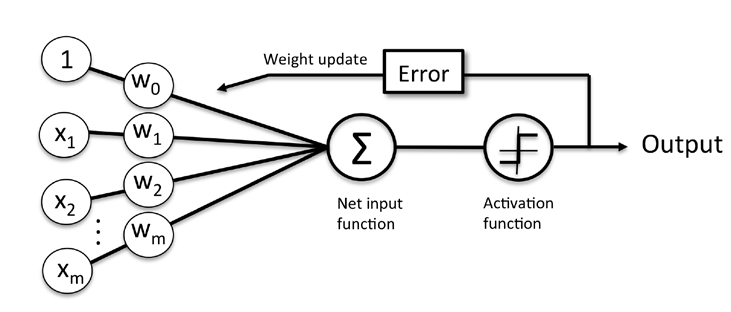
\includegraphics[width=.9\linewidth]{images/perceptron-summary.png}
\end{center}
\end{frame}

\begin{frame}[label={sec:orgeed2154}]{El perceptrón multicapa}
\begin{center}
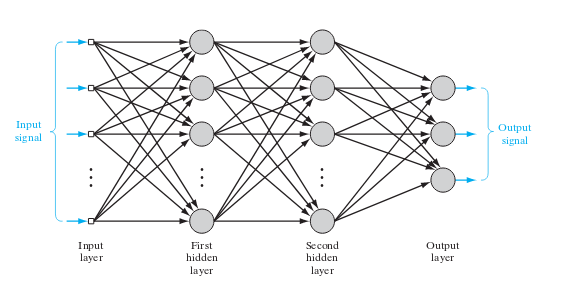
\includegraphics[width=.9\linewidth]{images/mlp.png}
\end{center}
\end{frame}
\begin{frame}[label={sec:org3ca0e72}]{El perceptrón multicapa}
\begin{center}
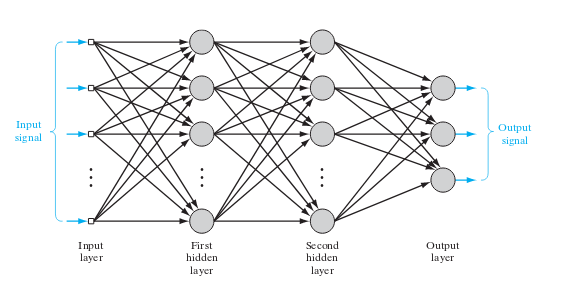
\includegraphics[width=170px]{images/mlp.png}
\end{center}
\begin{block}{Función de costo o error}
Definimos la función de costo \alert{\(J\)} para el perceptrón multicapa
como la suma de los errores cuadrados entre la salida calculada y
el valor real:
\begin{equation*}
J(w)=1/2n \sum_{i=1}^n (\hat{y}_i - y_i^2)
\end{equation*}

\pause
\begin{center}
¡Es diferenciable!
\end{center}
\end{block}
\end{frame}
\begin{frame}[label={sec:org6f25143}]{Descenso por el gradiente}
\begin{center}
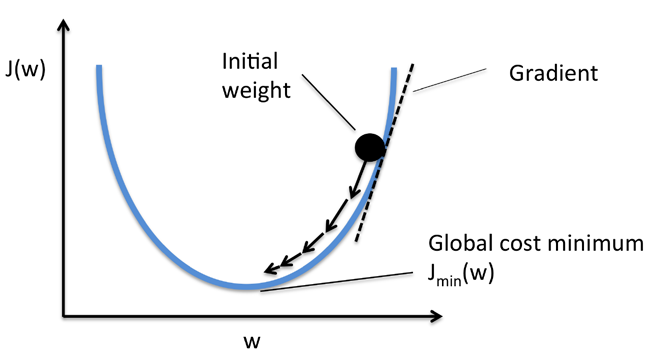
\includegraphics[width=.9\linewidth]{images/gradient-descent.png}
\end{center}
\end{frame}
\end{document}
